\section{Example}
\label{sec:example}

\begin{figure}[t]
\centering
\includegraphics[scale=0.8,clip]{figure/dataflow.eps}\vspace*{-3ex}
 \caption
{\label{fig:dataflow}API methods connected by inputs and
outputs}\vspace*{-2ex}
\end{figure}

In this section, we use an example to illustrate challenges of
mining API mapping. Suppose that a programmer need to migrate the
following code snippet from Java to C\# using a translation tool.

\begin{figure}[t]
\begin{CodeOut}
\begin{alltt}
1  File file = \textbf{new} File("test");
2    \textbf{if}(file.exists())\{...\}
\end{alltt}
\end{CodeOut}\vspace*{-4ex}
\caption{\label{fig:totranslation} A code example for language migration.}\vspace*{-4ex}
\end{figure}

The input of the code snippet is a string that denotes the name of a
file or a directory. The output of the code snippet is a boolean
value that denotes whether the file or the directory exists. To
achieve this functionality, the code snippet declares a local
variable whose type is \CodeIn{java.io.File} and calls
\CodeIn{exists()} of the local variable. Here, as \CodeIn{exists()}
is called through \CodeIn{file}, we call \CodeIn{file} as a receiver
of \CodeIn{exists()}. To translate this code snippet, a translation
tool needs to know mapping relations of API class to translate the
variable \CodeIn{file} to C\#. In addition, a translation tool needs
to know how to call API methods to use the variable and the input
(``\CodeIn{test}'') to produce the exactly same output.

As APIs are often large in size, a translation tool often supports
only a subset of mapping relations of used APIs. Thus, a translation
tool fails to translate the preceding code snippet correctly if the
translation tool does not support the preceding two API methods.
Some translation tools provide extensions for the programmer to add
customized rules for translation. To write a customized rule, a
programmer needs to know the mapping relation of APIs. Otherwise,
the programmer may choose to learn the mapping relation of APIs from
existing samples.

Many projects such as Lucene provide both C\# versions and Java
versions, and these projects provide various such samples. However,
it is not straightforward to learn those mapping relations of APIs.
The programmer needs to find Java source files that implement the
same functionality with the same input and output. For this example,
the programmer may find \CodeIn{IndexFiles.java} in the Java version
of Lucene useful as the file satisfies the preceding criteria. The
programmer then finds the corresponding source file
\CodeIn{IndexFiles.cs} from the C\# version of Lucene. The two files
are as follows:

\begin{figure}[t]
\begin{CodeOut}\vspace*{-2ex}
\begin{alltt}
                  IndexFiles.java
3 public class IndexFiles \{
4   static final File INDEX_DIR = new File("index");
5   public static void main(String[] args) \{
      ...
6     if (INDEX_DIR.exists()) \{...\}
      ...
7       INDEX_DIR.delete();
    \}
  \}
                  IndexFiles.cs
8 class IndexFiles\{
9   internal static readonly System.IO.FileInfo INDEX_DIR
          = new System.IO.FileInfo("index");
10   public static void  Main(System.String[] args)\{
      ...
11     bool tmpBool;
12     if (System.IO.File.Exists(INDEX_DIR.FullName))
13       tmpBool = true;
14    else
15       tmpBool = System.IO.Directory
                         .Exists(INDEX_DIR.FullName);
      ...
    \}
 \}
\end{alltt}
\end{CodeOut}\vspace*{-1ex}
\caption{\label{fig:clientcode} Two versions (Java and C\#) of client code.}\vspace*{-1ex}
\end{figure}

\begin{figure}[t]
\centering
\includegraphics[scale=0.65,clip]{figure/sample.eps}\vspace*{-3ex}
 \caption
{\label{fig:example}API mapping}\vspace*{-2ex}
\end{figure}

It is time-consuming to find out the two files as the two versions
of Lucene have more than 1,000 classes totally. Even after the
programmer successfully finds out the two aligned files, it is still
non-trivial to learn mapping relations of APIs. The programmer first
needs to map inputs of the three code snippets. In particular, by
comparing Line 1 with Line 4, the programmer knows that
\CodeIn{index} is the name for a file or a directory. Consequently,
the programmer analyzes how \CodeIn{index} in Line 4 (Java code) and
\CodeIn{index} in Line 9 (C\# code) are used in the two source files
for API mapping of interest so that boolean values are produced for
the functionality. To achieve so, the programmer chooses to analyze
inputs and outputs of each API method. Figure~\ref{fig:dataflow}
shows API methods connected by inputs and outputs for the preceding
two files. In particular, a box denotes an API method, and an
ellipse denotes either an input or an output. The strategy of
analyzing inputs and outputs helps find out an API method like
\CodeIn{System.IO.Directory.Exists()}. This API method is called in
an assignment statement, whereas three other related API methods are
called in infix expressions of if-statements. If the programmer
relies on call-site structures only, the programmer can miss the API
method as its call-site structure is quite different. To match
outputs, the programmer must know the mapping relations of classes.
For this example, the programmer should know the mapping relation
between \CodeIn{boolean} in Java and \CodeIn{System.Boolean}. After
the inputs and outputs are mapped, the programmer needs to further
match functionalities. For this example, the \CodeIn{delete()}
branch of Figure~\ref{fig:dataflow} implements a different
functionality as indicated by its name, and thus this branch is not
mapped with other branches.

The programmer learns mapping relations of APIs from the preceding
analysis. However, the analysis is not accurate enough. In
particular, Figure~\ref{fig:dataflow} does not consider parameters
and fails to provide useful information if two API methods have
different parameter orders. For this example, as shown in Line 6,
the input of \CodeIn{java.io.File.exist()} is a variable, but the
inputs of \CodeIn{Sys- tem.IO.Directory.Exist()} and
\CodeIn{System.IO.File.Exist()} are both their parameters as shown
in Line 12 and Line 15. The preceding analysis does not consider
parameters yet.

In this paper, we propose a novel approach that mines API mapping
automatically. Figure~\ref{fig:example} show the mined mapping
relation of APIs from the preceding two source files. In this
figure, a box denotes an API method. Here, our approach uses
\CodeIn{getFullName()} to denote the field access of
\CodeIn{FullName}. An ellipse denotes a parameter, a variable, or a
return value. Each ellipse is named as ``\emph{name:type}''. Here,
our approach uses ``variable'' for accesses of variables, ``null''
for return values, and parameter names for parameters.


The mined API mapping has matched inputs, outputs, and how inputs
and outputs are connected. Consequently, with the mined API mapping,
a translation tool can automatically translate the preceding code
snippet into C\# as follows:

\begin{figure}[t]
\begin{CodeOut}\vspace*{-1ex}
\begin{alltt}
16  FileInfo file = \textbf{new} FileInfo("test");
17  \textbf{if}(System.IO.File.Exist(file.FullName)||
       System.IO.Directory.Exists(file.FullName))\{...\}
\end{alltt}
\end{CodeOut}\vspace*{-1ex}
\caption{\label{fig:translatedcode} A translated code snippet from Java to C\#.}\vspace*{-1ex}
\end{figure}

In summary, for this example, we find that a programmer need to take
tedious and error-prone efforts to find and to analyze source files
from two versions of a project for API mapping. We next present our
approach to mine API mapping automatically.
%Based on the mapping relations, a translation tool can migrate the
%preceding code snippet automatically. To learn the mapping
%relations,
%
%%\begin{figure}[t]
%%\centering
%%\includegraphics[scale=0.86,clip]{figure/openfile.eps}\vspace*{-1.5ex}
%% \caption
%%{\label{fig:openfile}Aligned client code}\vspace*{-2ex}
%%\end{figure}
%
%In this section, we illustrate the main steps of our approach to
%mine the API mapping in Java for \CodeIn{System.IO.Directory.
%Exists()} in C\# from the HypoLog
%project\footnote{\url{http://sourceforge.net/projects/twlog/}}.
%
%The first step of our approach is to align classes and methods of
%client code by names. This step finds class pairs and method pairs
%that implement similar functionalities, and each pair may use
%API mapping since it implements a similar functionality. Our
%approach chooses names to align classes and methods because these
%classes and methods are from the same project. In this example, our
%approach aligns the two methods as shown in
%Figure~\ref{fig:openfile} because the two method have similar names
%and their declaring classes also have similar names (see
%Section~\ref{sec:approach:alignclientcode} for details).
%
%The second step of our approach is to mine mapping relations of API
%classes based on the names of corresponding fields, parameters,
%returned types, and local variables. This step also relies on names
%for the same consideration of the first step. For example, our
%approach maps the two parameters with the same name as shown by the
%red arrow of Figure~\ref{fig:openfile}. From the types of the two
%parameters, our approach mines the mapping relation between two API
%classes: \CodeIn{System.String} $\leftrightarrow$
%\CodeIn{java.lang.String} (see
%Section~\ref{sec:approach:mappingtypes} for details).
%
%
%The final step of our approach is to mine mapping relations of API
%methods. Besides the factors listed in
%Section~\ref{sec:introduction}, another factor is that API calls in
%client code are often not carefully aligned. To deal with those
%challenges, our approach first builds an API Transformation Graph
%(ATG) for each method. After that, our approach compares built
%graphs to mine mapping relations of API methods (see
%Section~\ref{sec:approach:mappingtypes} and
%Figure~\ref{fig:approach1} for details). Figure~\ref{fig:example}
%shows the mined mapping relation between
%\CodeIn{System.IO.Directory.Exists()} and its API mapping in
%Java.
